\chapter{Reacciones pericíclicas}\label{ch:b3:pericyclic}

La luz solar que incide sobre la piel abre un anillo del 7-deshidrocolesterol en una fracción
de segundo; el calor del cuerpo desplaza después un átomo de hidrógeno a través de siete átomos de carbono,
y el producto es la vitamina D$_3$. Ninguna de las dos etapas tiene intermedio: los enlaces se rompen
y se forman a la vez, alrededor de un anillo de átomos, a lo largo de un único estado de transición. La
primera etapa solo ocurre con luz y la segunda solo con calor, y cada una da
un único estereoisómero. Este capítulo explica por qué, a partir de la simetría de los
orbitales moleculares implicados: las reglas descubiertas por Robert Woodward y Roald
Hoffmann, que predicen si una reacción así puede ocurrir y qué da.

\begin{recall}
El volumen del segundo año dio los coeficientes de Hückel de los polienos, los anillos aromáticos y
antiaromáticos, la HOMO, la LUMO y los orbitales frontera, las reacciones concertadas y
la reacción de Diels--Alder de un dieno con un dienófilo con su regla endo; el
volumen del primer año, los descriptores \textit{Z}/\textit{E}. El \cref{ch:b3:point-groups} definió el eje $C_2$
y el \omterm{def:b3:point-groups:mirror}{plano de simetría}, y el \cref{ch:b3:photochemistry}, los estados excitados y la
fotocicloadición [2+2].
\end{recall}

\begin{omfigure}
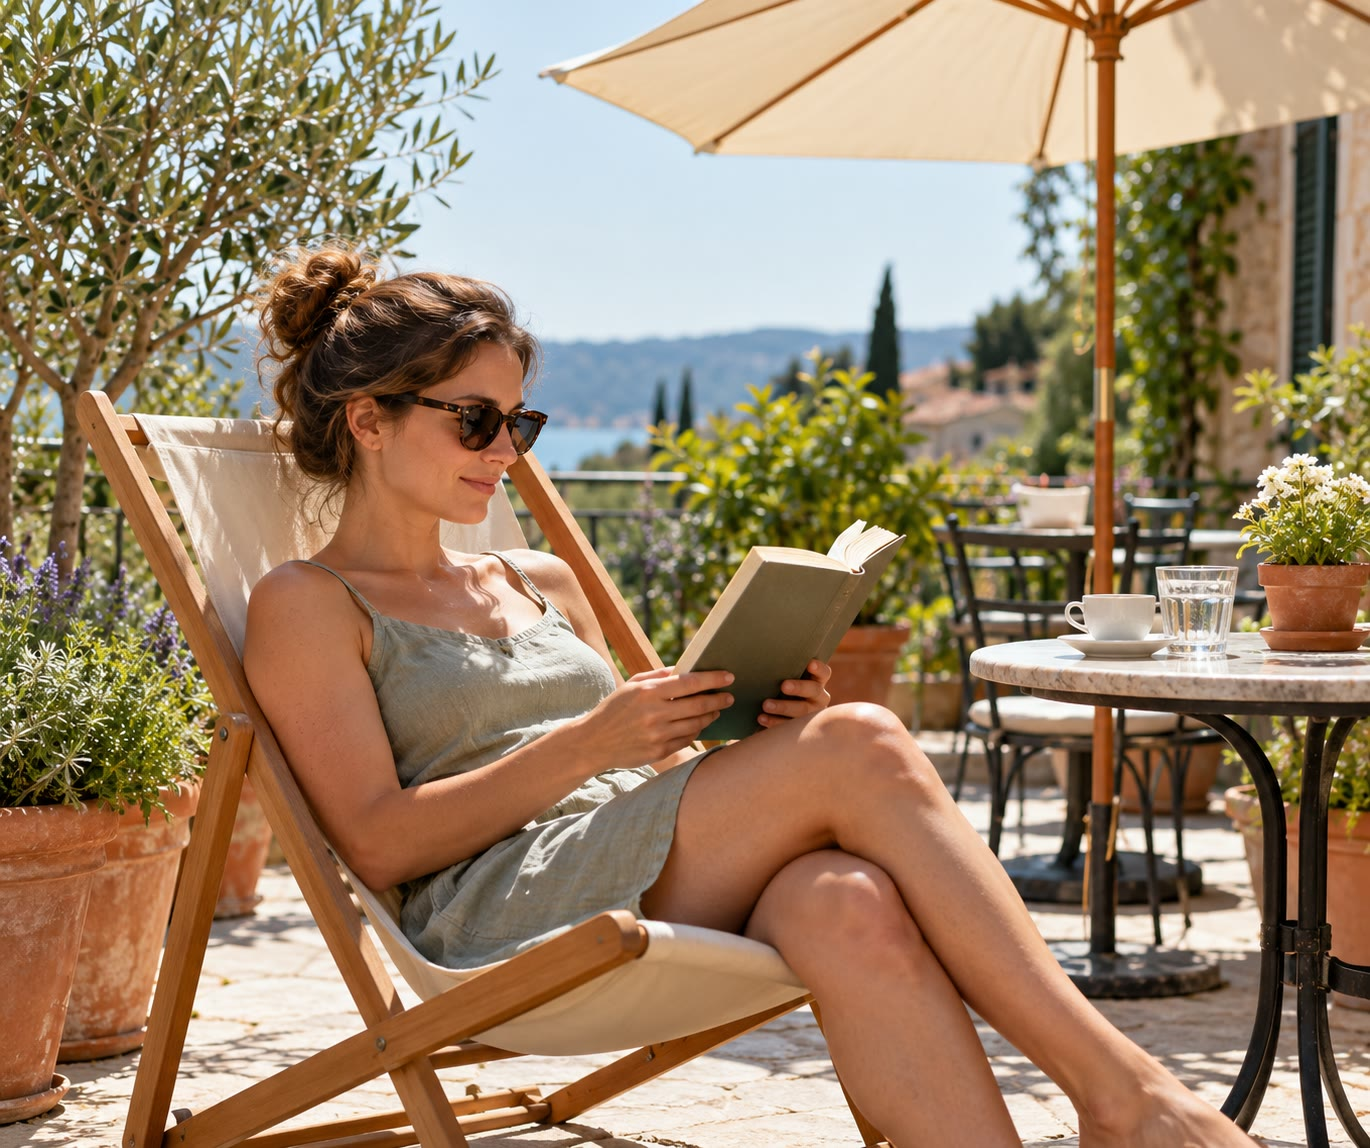
\includegraphics[width=0.55\linewidth]{images/book4/ai/b3-26-terrace.jpg}

{\small Lectura en una terraza soleada: la luz ultravioleta que llega a la piel inicia
la síntesis de la vitamina D$_3$ con una apertura de anillo pericíclica.}
\end{omfigure}

\section{Cuatro familias}

\begin{definition}[Reacción pericíclica]\label{def:b3:pericyclic:pericyclic}
Una \emph{reacción pericíclica}\index{reaccion periciclica@reacción pericíclica} es una reacción concertada
cuyo estado de transición es una disposición cíclica de orbitales en interacción, en la que todos
los enlaces se forman y se rompen alrededor del anillo al mismo tiempo.
\end{definition}

\begin{definition}[Familias de reacciones pericíclicas]\label{def:b3:pericyclic:families}
En una \emph{reacción electrocíclica}\index{reaccion electrociclica@reacción electrocíclica}, un polieno
conjugado se cierra en un anillo formando un enlace $\sigma$ entre sus extremos, o a la
inversa. En una \emph{cicloadición}\index{cicloadicion@cicloadición}, dos sistemas $\pi$ se unen
en un anillo formando dos enlaces $\sigma$; una cicloadición $[m + n]$ une componentes
de $m$ y $n$ átomos (o electrones). En una \emph{transposición
sigmatrópica}\index{transposicion sigmatropica@transposición sigmatrópica}, un enlace $\sigma$ migra a lo largo de un sistema
$\pi$; en un desplazamiento $[i, j]$, el enlace pasa de los átomos 1 y 1 a los átomos $i$ y $j$
de los dos fragmentos. Una \emph{reacción queletrópica}\index{reaccion queletropica@reacción queletrópica}
forma o rompe dos enlaces con un mismo átomo, como cuando el dióxido de azufre
abandona un sulfoleno. En una \emph{reacción eno}\index{reaccion eno@reacción eno}, un alqueno
con un hidrógeno alílico se adiciona a un enlace $\pi$, y el hidrógeno se desplaza con él.
\end{definition}

\begin{definition}[Suprafacial y antarafacial]\label{def:b3:pericyclic:faciality}
Un componente reacciona \emph{suprafacialmente}\index{suprafacial} cuando sus dos nuevos
enlaces se forman, o sus dos enlaces antiguos se rompen, en la misma cara de su sistema $\pi$ (o con
retención en un enlace $\sigma$), y \emph{antarafacialmente}\index{antarafacial} cuando
están en caras opuestas (o con inversión).
\end{definition}

\section{Reacciones electrocíclicas}

\begin{definition}[Conrotatorio y disrotatorio]\label{def:b3:pericyclic:rotation-modes}
En un cierre de anillo electrocíclico, los dos grupos terminales giran en torno a los enlaces
que los unen a la cadena. La rotación es \emph{conrotatoria}\index{conrotatorio}
cuando ambos giran en el mismo sentido (ambos en el sentido de las agujas del reloj vistos a lo largo de la cadena), y
\emph{disrotatoria}\index{disrotatorio} cuando giran en sentidos opuestos.
\end{definition}

\begin{theorem}[Reacciones electrocíclicas]\label{thm:b3:pericyclic:electrocyclic}
Una \omterm{def:b3:pericyclic:families}{reacción electrocíclica} térmica de un polieno con $4n$ electrones $\pi$ es
\omterm{def:b3:pericyclic:rotation-modes}{conrotatoria}, y con $4n + 2$ electrones $\pi$, \omterm{def:b3:pericyclic:rotation-modes}{disrotatoria}.
\end{theorem}

\begin{proof}
El nuevo enlace $\sigma$ se forma a partir de los orbitales p terminales de la HOMO, que en la
reacción térmica contiene los electrones de mayor energía; solo es enlazante si los
lóbulos que giran hasta quedar enfrentados tienen el mismo signo. Por la fórmula de Hückel
(\cref{ch:b3:solid-state}), los coeficientes del orbital $k$ de una cadena de $N$ átomos son
proporcionales a $\sin(jk\pi/(N + 1))$, de modo que los dos extremos, $j = 1$ y $j = N$, tienen los
coeficientes $\sin(k\pi/(N + 1))$ y $\sin(Nk\pi/(N + 1)) = (-1)^{k+1}\sin(k\pi/(N + 1))$: el mismo signo para $k$ impar y
signos opuestos para $k$ par. Con $N$ átomos y $N$ electrones, la HOMO es
$k = N/2$. Para $N = 4n$, $k = 2n$ es par: los lóbulos superiores de los extremos tienen signos
opuestos, y los dos extremos deben girar en el mismo sentido, llevando cada uno hacia dentro su lóbulo
del signo que coincide: \omterm{def:b3:pericyclic:rotation-modes}{conrotatorio}. Para $N = 4n + 2$, $k = 2n + 1$ es impar: los lóbulos superiores
tienen el mismo signo, y girarlos uno hacia el otro es \omterm{def:b3:pericyclic:rotation-modes}{disrotatorio}.
\end{proof}

\begin{omfigure}
\begin{tikzpicture}[font=\small, >=Stealth]
  % butadiene HOMO psi2: 0.60 0.37 -0.37 -0.60 (lobes scaled x1.6)
  \foreach \x/\c in {0/0.60, 1/0.37, 2/-0.37, 3/-0.60} {
    \pic at (\x,0) {omp={1.6*\c}{90}};
    \fill (\x,0) circle (1.2pt);
  }
  \draw[black!60] (0,0) -- (3,0);
  \draw[->, thick, omThm] (-0.45,0.55) arc[start angle=130, end angle=20, radius=0.7];
  \draw[->, thick, omThm] (2.55,0.55) arc[start angle=130, end angle=20, radius=0.7];
  \node[font=\scriptsize, align=center] at (1.5,-1.3) {butadieno, $\psi_2$ (HOMO, 4 electrones):\\ extremos de signo opuesto: \textbf{conrotatorio}};
  \begin{scope}[xshift=6.2cm]
  % hexatriene HOMO psi3: 0.52 0.23 -0.42 -0.42 0.23 0.52
  \foreach \x/\c in {0/0.52, 0.8/0.23, 1.6/-0.42, 2.4/-0.42, 3.2/0.23, 4.0/0.52} {
    \pic at (\x,0) {omp={1.6*\c}{90}};
    \fill (\x,0) circle (1.2pt);
  }
  \draw[black!60] (0,0) -- (4.0,0);
  \draw[->, thick, omThm] (-0.45,0.55) arc[start angle=130, end angle=20, radius=0.7];
  \draw[->, thick, omThm] (4.45,0.55) arc[start angle=50, end angle=160, radius=0.7];
  \node[font=\scriptsize, align=center] at (2.0,-1.3) {hexatrieno, $\psi_3$ (HOMO, 6 electrones):\\ extremos del mismo signo: \textbf{disrotatorio}};
  \end{scope}
\end{tikzpicture}

{\small La HOMO del butadieno y la del hexatrieno, con los lóbulos escalados según sus
coeficientes de Hückel (azul y naranja: los dos signos), dibujadas a lo largo de la cadena.
Para que se forme un enlace entre los extremos, los lóbulos que giran hasta quedar enfrentados
deben tener el mismo signo: ambos extremos giran en el sentido de las agujas del reloj en el butadieno, y en sentidos
opuestos en el hexatrieno (flechas rojas).}
\end{omfigure}

La regla es estereoespecífica. El (\textit{E},\textit{E})-hexa-2,4-dieno, calentado, se cerraría
de forma \omterm{def:b3:pericyclic:rotation-modes}{conrotatoria} en \textit{trans}-3,4-dimetilciclobuteno; en la práctica, el
ciclobuteno, tensionado, es el que se abre, y el \textit{cis}-3,4-dimetilciclobuteno se abre
de forma \omterm{def:b3:pericyclic:rotation-modes}{conrotatoria} dando únicamente (\textit{E},\textit{Z})-hexa-2,4-dieno. El (\textit{E},\textit{Z},\textit{E})-octa-2,4,6-trieno se cierra
de forma \omterm{def:b3:pericyclic:rotation-modes}{disrotatoria} en \textit{cis}-5,6-dimetilciclohexa-1,3-dieno.

\begin{proposition}[Reacciones electrocíclicas fotoquímicas]\label{prop:b3:pericyclic:photo-electrocyclic}
Con luz, las reglas se invierten: $4n$ electrones, \omterm{def:b3:pericyclic:rotation-modes}{disrotatoria}; $4n + 2$, \omterm{def:b3:pericyclic:rotation-modes}{conrotatoria}.
\end{proposition}

\begin{proof}
La absorción de un fotón promueve un electrón de la HOMO, $k = N/2$, a la LUMO, $k = N/2 + 1$
(\cref{ch:b3:photochemistry}), que pasa a ser el orbital ocupado más alto y
controla los extremos. Su $k$ tiene la paridad opuesta, de modo que el signo relativo de sus
coeficientes terminales se invierte, y con él el sentido de rotación.
\end{proof}

\begin{method}[Predecir la estereoquímica de una reacción electrocíclica]\label{met:b3:pericyclic:predict-stereo}
\begin{enumerate}
  \item Contar los electrones $\pi$ del polieno de cadena abierta ($4n$ o $4n + 2$); anotar si hay calor o
        luz.
  \item Leer el modo: térmico, $4n$ con, $4n + 2$ dis; fotoquímico, a la inversa.
  \item Dibujar los extremos con sus sustituyentes, en la conformación que
        se cierra (s-cis); girarlos 90° en el modo elegido.
  \item Leer si los dos sustituyentes acaban en la misma cara del anillo
        (\textit{cis}) o en caras opuestas (\textit{trans}). Para una apertura de anillo, hacer el mismo
        análisis en sentido inverso.
\end{enumerate}
\end{method}

\section{Diagramas de correlación orbital}

El argumento original de Woodward y Hoffmann examina todos los orbitales, no solo
la HOMO. A lo largo de un camino \omterm{def:b3:pericyclic:rotation-modes}{conrotatorio}, la molécula conserva un eje $C_2$; a lo largo de un
camino \omterm{def:b3:pericyclic:rotation-modes}{disrotatorio}, un \omterm{def:b3:point-groups:mirror}{plano de simetría} $\sigma$. Cada orbital del reactivo y del
producto es simétrico (S) o antisimétrico (A) respecto del elemento que
se conserva.

\begin{definition}[Diagrama de correlación orbital]\label{def:b3:pericyclic:orbital-correlation}
Un \emph{diagrama de correlación orbital}\index{diagrama de correlacion orbital@diagrama de correlación orbital} une
cada orbital del reactivo con el orbital del producto de la misma simetría,
respecto de los \omterm{def:b3:point-groups:operation}{elementos de simetría} conservados a lo largo del camino de reacción, tomándolos
por orden de energía: el S más bajo con el S más bajo, y así sucesivamente.
\end{definition}

\begin{proposition}[Conservación de la simetría orbital]\label{prop:b3:pericyclic:correlation}
Si todo orbital ocupado del reactivo se correlaciona con un orbital ocupado del
producto, la reacción térmica está permitida; si un orbital ocupado se correlaciona
con uno vacío, está prohibida, con una barrera alta.
\end{proposition}

\begin{proof}[Argumento]
A lo largo del camino, un orbital conserva su simetría y su energía varía de forma
continua; los orbitales de la misma simetría no pueden cruzarse (se mezclan y se repelen),
y los de simetría distinta sí. Cuando un orbital doblemente ocupado del reactivo
debe convertirse en un orbital antienlazante del producto, el estado fundamental del
reactivo conduce a un estado doblemente excitado del producto, y la energía del estado fundamental
sube bruscamente hasta que, al final del camino, los estados de la misma simetría
se mezclan: la barrera es alta.
\end{proof}

\begin{omfigure}
\begin{tikzpicture}[font=\scriptsize]
  \foreach \px/\title/\el in {0/disrotatorio: $\sigma$ conservado/s, 7.6/conrotatorio: $C_2$ conservado/c} {
    \begin{scope}[xshift=\px cm]
    \node[font=\small\bfseries] at (2.0,5.1) {\title};
    \node at (0,4.7) {butadieno};
    \node at (4.0,4.7) {ciclobuteno};
    \end{scope}
  }
  % ---- disrotatory (mirror): butadiene psi1 S, psi2 A, psi3 S, psi4 A;
  %      cyclobutene sigma S, pi S, pi* A, sigma* A
  \pic (b1) at (0,0.6) {omlevel={ud}{1.0}}; \node[anchor=east] at (-0.6,0.6) {$\psi_1$ S};
  \pic (b2) at (0,1.8) {omlevel={ud}{1.0}}; \node[anchor=east] at (-0.6,1.8) {$\psi_2$ A};
  \pic (b3) at (0,3.0) {omlevel={}{1.0}}; \node[anchor=east] at (-0.6,3.0) {$\psi_3$ S};
  \pic (b4) at (0,4.1) {omlevel={}{1.0}}; \node[anchor=east] at (-0.6,4.1) {$\psi_4$ A};
  \pic (c1) at (4.0,0.1) {omlevel={ud}{1.0}}; \node[anchor=west] at (4.6,0.1) {$\sigma$ S};
  \pic (c2) at (4.0,1.3) {omlevel={ud}{1.0}}; \node[anchor=west] at (4.6,1.3) {$\pi$ S};
  \pic (c3) at (4.0,3.4) {omlevel={}{1.0}}; \node[anchor=west] at (4.6,3.4) {$\pi^*$ A};
  \pic (c4) at (4.0,4.4) {omlevel={}{1.0}}; \node[anchor=west] at (4.6,4.4) {$\sigma^*$ A};
  \draw[omcorr] (b1-r) -- (c1-l);
  \draw[omcorrforbidden] (b2-r) -- (c3-l);
  \draw[omcorr] (b3-r) -- (c2-l);
  \draw[omcorr] (b4-r) -- (c4-l);
  % ---- conrotatory (C2): butadiene psi1 A, psi2 S, psi3 A, psi4 S;
  %      cyclobutene sigma S, pi A, pi* S, sigma* A
  \begin{scope}[xshift=7.6cm]
  \pic (d1) at (0,0.6) {omlevel={ud}{1.0}}; \node[anchor=east] at (-0.6,0.6) {$\psi_1$ A};
  \pic (d2) at (0,1.8) {omlevel={ud}{1.0}}; \node[anchor=east] at (-0.6,1.8) {$\psi_2$ S};
  \pic (d3) at (0,3.0) {omlevel={}{1.0}}; \node[anchor=east] at (-0.6,3.0) {$\psi_3$ A};
  \pic (d4) at (0,4.1) {omlevel={}{1.0}}; \node[anchor=east] at (-0.6,4.1) {$\psi_4$ S};
  \pic (e1) at (4.0,0.1) {omlevel={ud}{1.0}}; \node[anchor=west] at (4.6,0.1) {$\sigma$ S};
  \pic (e2) at (4.0,1.3) {omlevel={ud}{1.0}}; \node[anchor=west] at (4.6,1.3) {$\pi$ A};
  \pic (e3) at (4.0,3.4) {omlevel={}{1.0}}; \node[anchor=west] at (4.6,3.4) {$\pi^*$ S};
  \pic (e4) at (4.0,4.4) {omlevel={}{1.0}}; \node[anchor=west] at (4.6,4.4) {$\sigma^*$ A};
  \draw[omcorr] (d1-r) -- (e2-l);
  \draw[omcorr] (d2-r) -- (e1-l);
  \draw[omcorr] (d3-r) -- (e4-l);
  \draw[omcorr] (d4-r) -- (e3-l);
  \end{scope}
\end{tikzpicture}

{\small \omterm{def:b3:pericyclic:orbital-correlation}{Diagramas de correlación orbital} del butadieno $\rightleftharpoons$ ciclobuteno. A la izquierda, el
camino \omterm{def:b3:pericyclic:rotation-modes}{disrotatorio} conserva un \omterm{def:b3:point-groups:mirror}{plano de simetría}: la $\psi_2$ (A) ocupada se correlaciona con el
$\pi^*$ (A) vacío del ciclobuteno (trazo discontinuo rojo): térmicamente prohibido. A la derecha, el
camino \omterm{def:b3:pericyclic:rotation-modes}{conrotatorio} conserva un eje $C_2$: los orbitales ocupados van a orbitales ocupados:
térmicamente permitido.}
\end{omfigure}

\begin{method}[Construir un diagrama de correlación]\label{met:b3:pericyclic:correlation-diagram}
\begin{enumerate}
  \item Encontrar los \omterm{def:b3:point-groups:operation}{elementos de simetría} que bisecan los enlaces que se forman y se rompen y que se
        conservan a lo largo de todo el camino elegido.
  \item Enumerar los orbitales que intervienen, del reactivo y del producto, por orden de
        energía, y etiquetar cada uno como S o A para cada elemento.
  \item Unir el orbital más bajo de cada tipo de simetría de un lado con el más bajo
        del mismo tipo del otro, después el siguiente, sin cruzar nunca dos líneas de la
        misma simetría.
  \item Comprobar los orbitales ocupados: todos hacia ocupados, permitida; uno hacia uno vacío,
        prohibida.
\end{enumerate}
\end{method}

\begin{definition}[Diagrama de correlación de estados]\label{def:b3:pericyclic:state-correlation}
Un \emph{diagrama de correlación de estados}\index{diagrama de correlacion de estados@diagrama de correlación de estados} une los
estados electrónicos del reactivo y del producto, construido cada uno a partir de las configuraciones
orbitales y etiquetado por su simetría global, a lo largo del camino; los estados de
la misma simetría no se cruzan.
\end{definition}

En el camino \omterm{def:b3:pericyclic:rotation-modes}{disrotatorio} prohibido, el estado fundamental del butadieno ($\psi_1^2\psi_2^2$)
se correlaciona con un estado doblemente excitado del ciclobuteno ($\sigma^2\pi^{*2}$), pero el primer estado
excitado ($\psi_1^2\psi_2\psi_3$) se correlaciona con el primer estado excitado del ciclobuteno ($\sigma^2\pi\pi^*$): desde el
estado excitado, el camino \omterm{def:b3:pericyclic:rotation-modes}{disrotatorio} es descendente. Es la inversión fotoquímica
de la \cref{prop:b3:pericyclic:photo-electrocyclic}, vista sobre los estados.

\section{Cicloadiciones}

\begin{theorem}[Cicloadiciones]\label{thm:b3:pericyclic:cycloaddition}
Una \omterm{def:b3:pericyclic:families}{cicloadición} $[m + n]$ térmica en la que ambos componentes reaccionan \omterm{def:b3:pericyclic:faciality}{suprafacialmente} está
permitida cuando $m + n = 4q + 2$ electrones, y prohibida cuando $m + n = 4q$; con luz, la
regla se invierte.
\end{theorem}

\begin{proof}
Los dos nuevos enlaces se forman entre la HOMO de un componente y la LUMO del
otro, que se enfrentan por sus lóbulos terminales; si ambos reaccionan
\omterm{def:b3:pericyclic:faciality}{suprafacialmente}, los dos enlaces solo son enlazantes si los coeficientes terminales de la
HOMO y de la LUMO tienen el mismo signo relativo. Para un componente de $N$
electrones sobre $N$ átomos, la HOMO tiene $k = N/2$, y la LUMO, $k = N/2 + 1$; los coeficientes terminales son del
mismo signo para $k$ impar y de signo opuesto para $k$ par. En el caso [4+2], la HOMO del dieno ($k = 2$)
y la LUMO del eteno ($k = 2$) tienen ambas signos terminales opuestos: coinciden. En el
caso [2+2], la HOMO de un eteno ($k = 1$, mismos signos) se encuentra con la LUMO del otro
($k = 2$, opuestos): un extremo enlazante y otro antienlazante. En general, la HOMO del componente $m$
y la LUMO del componente $n$ coinciden cuando $m/2$ y $n/2 + 1$ tienen la misma
paridad, es decir, cuando $(m + n)/2$ es impar: $m + n = 4q + 2$. Con luz, la LUMO simplemente ocupada del
componente excitado desempeña el papel de su HOMO, y la condición de paridad se
invierte.
\end{proof}

\begin{omfigure}
\begin{tikzpicture}[font=\scriptsize]
  % [4+2]: diene HOMO above, ethene LUMO (pi*) below, facing lobes match at both ends
  \foreach \x/\c in {0/0.60, 1/0.37, 2/-0.37, 3/-0.60} {
    \pic at (\x,1.6) {omp={1.4*\c}{90}}; \fill (\x,1.6) circle (1.1pt);
  }
  \draw[black!60] (0,1.6) -- (3,1.6);
  \foreach \x/\c in {0/-0.71, 3/0.71} {
    \pic at (\x,-0.4) {omp={1.4*\c}{90}}; \fill (\x,-0.4) circle (1.1pt);
  }
  \draw[black!60] (0,-0.4) -- (3,-0.4);
  \draw[omMeth, densely dashed, thick] (-0.25,0.75) -- (-0.25,0.35) (3.25,0.75) -- (3.25,0.35);
  \node[omMeth] at (-0.25,0.55) [left] {enlazante};
  \node[omMeth] at (3.25,0.55) [right] {enlazante};
  \node[font=\small] at (1.5,2.95) {[4+2]: HOMO del dieno};
  \node[font=\small] at (1.5,-1.75) {LUMO del eteno: permitida};
  \begin{scope}[xshift=7.2cm]
  \foreach \x/\c in {0/0.71, 3/0.71} {
    \pic at (\x,1.6) {omp={1.4*\c}{90}}; \fill (\x,1.6) circle (1.1pt);
  }
  \draw[black!60] (0,1.6) -- (3,1.6);
  \foreach \x/\c in {0/-0.71, 3/0.71} {
    \pic at (\x,-0.4) {omp={1.4*\c}{90}}; \fill (\x,-0.4) circle (1.1pt);
  }
  \draw[black!60] (0,-0.4) -- (3,-0.4);
  \draw[omMeth, densely dashed, thick] (-0.25,0.75) -- (-0.25,0.35);
  \draw[omThm, densely dashed, thick] (3.25,0.75) -- (3.25,0.35);
  \node[omMeth] at (-0.25,0.55) [left] {enlazante};
  \node[omThm] at (3.25,0.55) [right] {antienlazante};
  \node[font=\small] at (1.5,2.95) {[2+2]: HOMO del eteno};
  \node[font=\small] at (1.5,-1.75) {LUMO del eteno: prohibida};
  \end{scope}
\end{tikzpicture}

{\small Orbitales frontera enfrentados en \omterm{def:b3:pericyclic:families}{cicloadiciones} \omterm{def:b3:pericyclic:faciality}{suprafaciales} (los
lóbulos inferiores del componente superior se encuentran con los lóbulos superiores del inferior; tamaños
de los lóbulos según los coeficientes de Hückel). En la reacción [4+2], los dos nuevos enlaces son
enlazantes; en la reacción [2+2], un extremo es enlazante y el otro antienlazante.}
\end{omfigure}

Por vía térmica, dos alquenos no dan un ciclobutano en una sola etapa concertada; con
luz, sí (\cref{ch:b3:photochemistry}). Los cetenos son la excepción que
confirma la regla: su orbital $\pi^*$ C=O, perpendicular al C=C, les permite
reaccionar con un alqueno en una geometría [$\pi2_s$ + $\pi2_a$], con un componente \omterm{def:b3:pericyclic:faciality}{suprafacial} y el
ceteno \omterm{def:b3:pericyclic:faciality}{antarafacial}, y forman ciclobutanonas por vía térmica.

\begin{definition}[Cicloadiciones 1,3-dipolares]\label{def:b3:pericyclic:dipolar}
Un \emph{1,3-dipolo}\index{1,3-dipolo} es un sistema $\pi$ de tres átomos con cuatro
electrones, escrito con cargas formales en sus extremos o en el centro, como una
azida $\ce{R-N=N+=N-}$, un óxido de nitrilo o una molécula de ozono. Una \emph{cicloadición
1,3-dipolar}\index{cicloadicion 1,3-dipolar@cicloadición 1,3-dipolar} es su \omterm{def:b3:pericyclic:families}{cicloadición} [3+2], una
reacción de seis electrones, con un alqueno o un alquino, que da un anillo de cinco miembros.
\end{definition}

La reacción catalizada por cobre de una azida con un alquino terminal, que da un solo
regioisómero de un 1,2,3-triazol, es la reacción de unión fiable de la química
\textit{click}. La ozonólisis comienza con una \omterm{def:b3:pericyclic:dipolar}{cicloadición 1,3-dipolar} del ozono al
alqueno.

\section{Transposiciones sigmatrópicas y la regla general}

\begin{proposition}[Desplazamientos de hidrógeno]\label{prop:b3:pericyclic:sigmatropic-h}
Un desplazamiento $[1, j]$ térmico de un hidrógeno a lo largo de un polieno está permitido \omterm{def:b3:pericyclic:faciality}{suprafacialmente} cuando el
estado de transición contiene $4q + 2$ electrones ($[1,5]$), y debe ser \omterm{def:b3:pericyclic:faciality}{antarafacial} cuando contiene $4q$
($[1,3]$, $[1,7]$).
\end{proposition}

\begin{proof}
Se trata el estado de transición como un átomo de hidrógeno (1s) que se desplaza entre los extremos de un
radical de $j$ átomos con $j$ electrones; el hidrógeno tiende un puente entre los dos extremos del
SOMO, $k = (j + 1)/2$. Para $j = 5$, $k = 3$ es impar, los extremos tienen lóbulos del mismo signo en una cara,
y el orbital 1s puede enlazarse a ambos por esa cara: \omterm{def:b3:pericyclic:faciality}{suprafacial}. Para $j = 3$ y $j = 7$,
$k = 2$ y $4$ son pares, los lóbulos del mismo signo están en caras opuestas en los dos extremos, y
el hidrógeno debe pasar de una cara a la otra: \omterm{def:b3:pericyclic:faciality}{antarafacial}. Un desplazamiento $[1,3]$
no puede alcanzar el otro extremo de una cadena tan corta; un desplazamiento $[1,7]$ sí, a lo largo de un polieno helicoidal.
\end{proof}

\begin{definition}[Transposiciones de Cope y de Claisen]\label{def:b3:pericyclic:cope-claisen}
La \emph{transposición de Cope}\index{transposicion de Cope@transposición de Cope} es la \omterm{def:b3:pericyclic:families}{transposición sigmatrópica} [3,3]
de un hexa-1,5-dieno; la \emph{transposición de
Claisen}\index{transposicion de Claisen@transposición de Claisen}, la de un alil vinil éter, o de
un alil aril éter, en un compuesto carbonílico $\gamma,\delta$-insaturado o en un \textit{orto}-alilfenol.
\end{definition}

\begin{omfigure}
\begin{tikzpicture}[font=\scriptsize, scale=1.1]
  \foreach \px/\three/\title in {0/C/Cope, 5.0/O/Claisen} {
    \begin{scope}[xshift=\px cm]
      % chair: atoms at 60-degree steps, alternately 0.25 above and below the
      % mean plane, seen from slightly above (y' = 0.35 y + z), scaled
      \begin{scope}[shift={(1.3,0.2)}, scale=1.15]
      \coordinate (a1) at (-1.25,-0.25); \coordinate (a2) at (-0.625,-0.129); \coordinate (a3) at (0.625,-0.629);
      \coordinate (a4) at (1.25,0.25); \coordinate (a5) at (0.625,0.129); \coordinate (a6) at (-0.625,0.629);
      \end{scope}
      \draw[thick] (a1) -- (a2) -- (a3);
      \draw[thick] (a4) -- (a5) -- (a6);
      \draw[omThm, thick, densely dashed] (a3) -- (a4);
      \draw[omMeth, thick, densely dashed] (a6) -- (a1);
      \foreach \i/\l in {1/1, 2/2, 4/4, 5/5, 6/6} { \fill (a\i) circle (1.3pt); }
      \node[fill=white, inner sep=0.6pt] at (a3) {\three};
      \node[anchor=east] at (a1) {1};
      \node[anchor=north] at (a2) {2};
      \node[anchor=north west] at (a3) {3};
      \node[anchor=west] at (a4) {4};
      \node[anchor=south] at (a5) {5};
      \node[anchor=south] at (a6) {6};
      \node[font=\small\bfseries] at (1.3,1.5) {\title};
    \end{scope}
  }
\end{tikzpicture}

{\small Estados de transición en silla de \omterm{def:b3:pericyclic:families}{transposiciones sigmatrópicas} [3,3]: dos fragmentos
alilo se enfrentan; el enlace $\sigma$ 3--4 se rompe (rojo) mientras se forma el enlace 1--6
(verde). En la \omterm{def:b3:pericyclic:cope-claisen}{transposición de Claisen}, el átomo 3 es el oxígeno del éter, y el
producto es un compuesto carbonílico. La silla fija la configuración relativa de los
nuevos estereocentros.}
\end{omfigure}

El desplazamiento [3,3] es un proceso de seis electrones, totalmente \omterm{def:b3:pericyclic:faciality}{suprafacial}, permitido por vía térmica;
transcurre a través de un estado de transición de tipo silla, como un ciclohexano, y
los sustituyentes prefieren sus posiciones ecuatoriales: los dienos (\textit{E},\textit{E}) y (\textit{Z},\textit{Z}) dan
configuraciones relativas opuestas, de forma previsible.

\begin{theorem}[Reglas de Woodward--Hoffmann]\label{thm:b3:pericyclic:woodward-hoffmann}
Una \omterm{def:b3:pericyclic:pericyclic}{reacción pericíclica} térmica está permitida cuando el número total de componentes $(4q + 2)_s$ y
$(4r)_a$ es impar; una fotoquímica, cuando es par.
\end{theorem}

\begin{proof}[Demostración parcial]
Para cada familia tratada antes, el recuento concuerda con el análisis de los orbitales
frontera: una \omterm{def:b3:pericyclic:families}{cicloadición} [4+2] térmica tiene los componentes $\pi4_s$ y $\pi2_s$, un componente $(4q + 2)_s$,
impar: permitida; la [2+2] tiene $\pi2_s + \pi2_s$, dos, par: prohibida, mientras que
$\pi2_s + \pi2_a$ tiene uno: permitida; la apertura \omterm{def:b3:pericyclic:rotation-modes}{conrotatoria} del ciclobuteno es $\sigma2_s + \pi2_a$, uno:
permitida; el desplazamiento $[1,5]$-H \omterm{def:b3:pericyclic:faciality}{suprafacial} es $\sigma2_s + \pi4_s$, donde solo cuenta $\sigma2_s$: uno,
permitido. La demostración general, válida para cualquier disposición de componentes, corresponde
a cursos más avanzados.
\end{proof}

\begin{definition}[Estados de transición aromáticos y de Möbius]\label{def:b3:pericyclic:mobius}
Un \emph{estado de transición aromático}\index{estado de transicion aromatico@estado de transición aromático} es una disposición
cíclica de orbitales en un estado de transición pericíclico que, como un anillo de Hückel, se
estabiliza cuando contiene $4q + 2$ electrones. Un \emph{estado de transición de
Möbius}\index{estado de transicion de Mobius@estado de transición de Möbius} tiene un número impar de cambios de signo entre
orbitales vecinos alrededor del anillo (una torsión \omterm{def:b3:pericyclic:faciality}{antarafacial}); se
estabiliza con $4q$ electrones.
\end{definition}

\begin{proposition}[Estados de transición aromáticos]\label{prop:b3:pericyclic:aromatic-ts}
Una \omterm{def:b3:pericyclic:pericyclic}{reacción pericíclica} térmica está permitida cuando su estado de transición es aromático:
topología de Hückel con $4q + 2$ electrones, o topología de Möbius con $4q$ electrones.
\end{proposition}

\begin{proof}[Argumento]
La disposición cíclica de orbitales del estado de transición se comporta como una molécula
conjugada cíclica. Un anillo de Hückel tiene su nivel más bajo no degenerado y pares de niveles
por encima, llenos con $4q + 2$ electrones (volumen del segundo año); un anillo con una inversión de
signo tiene todos sus niveles por pares, llenos con $4q$. Una capa llena significa
estabilización, un \omterm{def:b3:pericyclic:mobius}{estado de transición aromático} y una barrera baja. El número de cambios
de signo es el número de componentes \omterm{def:b3:pericyclic:faciality}{antarafaciales}, de modo que esta regla equivale a la
regla de Woodward--Hoffmann.
\end{proof}

\begin{method}[Dibujar y contar los componentes]\label{met:b3:pericyclic:components}
\begin{enumerate}
  \item Marcar los enlaces que se forman y se rompen; cada sistema $\pi$ o enlace $\sigma$ que cambia es un
        componente, etiquetado con su tipo y su número de electrones ($\pi4$, $\pi2$, $\sigma2$, $\omega0$ para
        un orbital vacío).
  \item Elegir s o a para cada componente según la geometría (misma cara o
        caras opuestas).
  \item Contar los componentes $(4q + 2)_s$ y $(4r)_a$: impar, permitida por vía térmica; par, permitida
        por vía fotoquímica.
  \item Comprobarlo con el número de electrones alrededor del anillo: Hückel con $4q + 2$,
        Möbius con $4q$.
\end{enumerate}
\end{method}

\begin{omfigure}
\begin{tikzpicture}[font=\scriptsize, >=Stealth]
  \foreach \px/\mode in {0/1, 4.6/2, 9.2/3} {
    \begin{scope}[xshift=\px cm]
      \foreach \n/\a in {10/210, 5/150, 6/90, 7/30, 8/-30, 9/-90} { \coordinate (v\n) at (\a:0.85); }
      \ifnum\mode=1
        \draw[thick] (v10) -- (v5) (v6) -- (v7) (v8) -- (v9);
        \draw[thick, double, double distance=1.6pt] (v5) -- (v6) (v7) -- (v8);
        \draw[thick, omThm] (v9) -- (v10);
        \draw[thick] (v10) -- ++(240:0.6) node[anchor=north] {$\ce{CH3}$};
        \node[font=\small\bfseries] at (0,1.55) {7-deshidrocolesterol};
      \fi
      \ifnum\mode=2
        \draw[thick, double, double distance=1.6pt] (v10) -- (v5) (v6) -- (v7) (v8) -- (v9);
        \draw[thick] (v5) -- (v6) (v7) -- (v8);
        \draw[thick] (v10) -- ++(240:0.6) node[anchor=north] (me) {$\ce{CH3}$};
        \draw[->, omThm, thick] ($(v10)+(240:0.75)+(0.35,0)$) to[bend right=40] ($(v9)+(-0.12,-0.12)$);
        \node[font=\small\bfseries] at (0,1.55) {previtamina D$_3$};
      \fi
      \ifnum\mode=3
        \draw[thick] (v10) -- (v5) (v6) -- (v7) (v8) -- (v9);
        \draw[thick, double, double distance=1.6pt] (v5) -- (v6) (v7) -- (v8);
        \draw[thick, double, double distance=1.6pt] (v10) -- ++(240:0.6) node[anchor=north] {$\ce{CH2}$};
        \node[anchor=north west, inner sep=1pt] at (v9) {$\ce{CH2}$};
        \node[font=\small\bfseries] at (0,1.55) {vitamina D$_3$};
      \fi
      \foreach \n/\a in {10/210, 5/150, 6/90, 7/30, 8/-30, 9/-110} {
        \node[font=\tiny, black!60] at (\a:1.12) {\n};
      }
    \end{scope}
  }
  \draw[->, thick] (1.45,0) -- (3.0,0) node[midway, above, align=center] {$h\nu$\\ 6 e$^-$, conrotatoria};
  \draw[->, thick] (6.05,0) -- (7.6,0) node[midway, above, align=center] {calor, $[1,7]$-H\\ antarafacial};
\end{tikzpicture}

{\small Las dos etapas pericíclicas de la síntesis de la vitamina D, dibujadas sobre los átomos
que reaccionan (numeración esteroidea en gris; se omite el resto de la molécula, los anillos A, C y D).
La luz abre el anillo B rompiendo el enlace 9--10 (rojo), una \omterm{def:b3:pericyclic:families}{reacción electrocíclica}
fotoquímica de seis electrones, \omterm{def:b3:pericyclic:rotation-modes}{conrotatoria}. En la previtamina D$_3$, un hidrógeno del
grupo metilo C19 se desplaza después a C9 (flecha roja) a través del trieno helicoidal
de siete átomos, de forma \omterm{def:b3:pericyclic:faciality}{antarafacial}.}
\end{omfigure}

\begin{inthelab}[Una transposición de Claisen]
Se calienta a reflujo un alil aril éter, bajo nitrógeno, en un disolvente de punto de ebullición
alto, como el 1,2-diclorobenceno, o sin disolvente, a unos \qty{200}{\celsius}, y
se sigue la reacción por cromatografía en capa fina: el \textit{orto}-alilfenol formado
es más polar que el éter. El fenol se extrae después en hidróxido de sodio acuoso,
se separa de las impurezas neutras y se recupera por acidificación.
\end{inthelab}

\begin{safety}{\ghs[0.62cm]{GHS02}\ghs[0.62cm]{GHS04}\ghs[0.62cm]{GHS08}}
% ledger: ghs4:butadiene
Buta-1,3-dieno, un dieno corriente: gas extremadamente inflamable a presión, puede provocar
defectos genéticos y cáncer. Solo se manipula en sistemas cerrados; en la enseñanza
se usa en su lugar, en un montaje cerrado, el sulfoleno sólido, que lo libera en una \omterm{def:b3:pericyclic:families}{reacción
queletrópica} al calentarlo.
\end{safety}

\begin{history}[La simetría orbital]
En 1965, Robert Woodward, que había encontrado la desconcertante estereoquímica de
etapas electrocíclicas mientras sintetizaba la vitamina B$_{12}$, y Roald Hoffmann publicaron
las reglas de conservación de la simetría orbital. Kenichi Fukui había introducido los
orbitales frontera en 1952; Fukui y Hoffmann compartieron el Premio Nobel de
Química de 1981. Woodward, que había recibido el premio de 1965 por sus síntesis, murió en
1979.
\end{history}

\section{Ejercicios}

\begin{exercise}[$\star$]\label{exo:b3:pericyclic:1}
Clasifíquense: la reacción de Diels--Alder; la apertura de anillo del ciclobuteno; la \omterm{def:b3:pericyclic:cope-claisen}{transposición
de Cope}; la pérdida de $\ce{SO2}$ del sulfoleno; la adición del ozono a un alqueno;
un desplazamiento $[1,5]$-H en el ciclopentadieno.
\end{exercise}

\begin{exercise}[$\star$]\label{exo:b3:pericyclic:2}
Predígase el modo, \omterm{def:b3:pericyclic:rotation-modes}{conrotatorio} o \omterm{def:b3:pericyclic:rotation-modes}{disrotatorio}, del cierre de anillo térmico y del
fotoquímico del hexa-1,3,5-trieno y del buta-1,3-dieno.
\end{exercise}

\begin{exercise}[$\star$]\label{exo:b3:pericyclic:3}
¿Qué producto da el \textit{trans}-3,4-dimetilciclobuteno al calentarlo?
\end{exercise}

\begin{exercise}[$\star$]\label{exo:b3:pericyclic:4}
¿Por qué el eteno no se dimeriza a ciclobutano al calentarlo, mientras que sí lo hace con luz
(con un \omterm{def:b3:photochemistry:sensitisation}{fotosensibilizador} o por excitación directa)?
\end{exercise}

\begin{exercise}[$\star\star$]\label{exo:b3:pericyclic:5}
Constrúyase el \omterm{def:b3:pericyclic:orbital-correlation}{diagrama de correlación orbital} hexatrieno $\rightleftharpoons$ ciclohexa-1,3-dieno para el
camino \omterm{def:b3:pericyclic:rotation-modes}{disrotatorio}, y extráigase una conclusión.
\end{exercise}

\begin{exercise}[$\star\star$]\label{exo:b3:pericyclic:6}
Con luz, ¿en qué dimetilciclohexadieno se cierra el (\textit{E},\textit{Z},\textit{E})-octa-2,4,6-trieno?
\end{exercise}

\begin{exercise}[$\star\star$]\label{exo:b3:pericyclic:7}
El 5-metilciclopenta-1,3-dieno se transpone a temperatura ambiente en 1- y
2-metilciclopentadienos. Explíquese con un desplazamiento $[1,5]$-H, y dígase por qué es \omterm{def:b3:pericyclic:faciality}{suprafacial}.
\end{exercise}

\begin{exercise}[$\star\star$]\label{exo:b3:pericyclic:8}
Cuéntense los componentes de la \omterm{def:b3:pericyclic:families}{cicloadición} de un ceteno a un alqueno, y demuéstrese
que está permitida por vía térmica.
\end{exercise}

\begin{exercise}[$\star\star$]\label{exo:b3:pericyclic:9}
El alil vinil éter, $\ce{CH2=CH-O-CH2-CH=CH2}$, experimenta la \omterm{def:b3:pericyclic:cope-claisen}{transposición de Claisen} al
calentarlo. Dibújese su estado de transición en silla y dese el producto.
\end{exercise}

\begin{exercise}[$\star\star\star$]\label{exo:b3:pericyclic:10}
Un estado de transición tiene ocho electrones en una disposición cíclica con un componente
\omterm{def:b3:pericyclic:faciality}{antarafacial}. ¿Es aromático? ¿Está permitida la reacción por vía térmica?
\end{exercise}

\begin{exercise}[$\star\star\star$]\label{exo:b3:pericyclic:11}
En la \omterm{def:b3:pericyclic:dipolar}{cicloadición 1,3-dipolar} de una azida con un alquino terminal, el mayor
coeficiente de la HOMO de la azida está en el nitrógeno terminal N3, y el mayor
coeficiente de la LUMO del alquino, en su carbono terminal (datos del ejercicio).
Predígase el regioisómero favorecido sin catalizador emparejando los mayores
coeficientes, y coméntese.
\end{exercise}

\begin{exercise}[$\star\star\star$]\label{exo:b3:pericyclic:12}
Demuéstrese, con la fórmula de Hückel, que el desplazamiento $[1,7]$-H debe ser \omterm{def:b3:pericyclic:faciality}{antarafacial},
y el desplazamiento $[1,5]$-H, \omterm{def:b3:pericyclic:faciality}{suprafacial}.
\end{exercise}

% keep the heading with its problem box, which fills a page by itself
\clearpage
\enlargethispage{3\baselineskip}
\section{Problema: luz solar, piel y vitamina D}

\begin{problem}[{Problema de fin de semana --- luz solar, piel y vitamina D: la
apertura de anillo fotoquímica del 7-deshidrocolesterol, el desplazamiento térmico de hidrógeno,
los productos secundarios y el tiempo que tarda el organismo en terminar el trabajo}]
\label{pb:b3:pericyclic:1}
Datos del problema: a \qty{37}{\celsius}, la conversión de la previtamina D$_3$ en vitamina D$_3$ es
de primer orden con $k = \qty{2.3e-2}{h^{-1}}$ (se desprecia la reacción inversa); su energía de activación es de
\qty{85}{kJ/mol}.

\medskip\noindent\textbf{Parte I --- La apertura de anillo.}
\begin{enumerate}
  \item ¿Qué enlace del 7-deshidrocolesterol se rompe, y qué sistema $\pi$ se forma?
  \item ¿Cuántos electrones intervienen, y a qué familia pertenece la reacción?
  \item ¿Por qué necesita luz?
  \item ¿Es la apertura fotoquímica \omterm{def:b3:pericyclic:rotation-modes}{conrotatoria} o \omterm{def:b3:pericyclic:rotation-modes}{disrotatoria}? Justifíquese con los
        orbitales.
  \item ¿Por qué debe ser \textit{Z} el nuevo doble enlace central de la previtamina D$_3$?
  \item ¿Por qué no puede darse la misma apertura térmicamente, a oscuras, a temperatura corporal?
\end{enumerate}

\medskip\noindent\textbf{Parte II --- El desplazamiento de hidrógeno.}
\begin{enumerate}[resume]
  \item Nómbrense los átomos entre los que se desplaza el hidrógeno, y el tipo de desplazamiento.
  \item ¿Cuántos electrones intervienen en el estado de transición?
  \item Cuéntense los componentes: ¿la reacción térmica permitida es \omterm{def:b3:pericyclic:faciality}{suprafacial}
        o \omterm{def:b3:pericyclic:faciality}{antarafacial}?
  \item ¿Por qué es aquí geométricamente posible un desplazamiento \omterm{def:b3:pericyclic:faciality}{antarafacial}, y uno $[1,3]$
        no?
  \item ¿Es el estado de transición de Hückel o de Möbius, y es aromático?
  \item ¿Por qué el desplazamiento no necesita luz?
\end{enumerate}

\medskip\noindent\textbf{Parte III --- Productos secundarios.}
\begin{enumerate}[resume]
  \item La previtamina D$_3$ puede volver a cerrarse con luz. ¿En qué modo, y por qué puede dar un
        estereoisómero de anillo del 7-deshidrocolesterol (lumisterol)?
  \item La luz también puede convertir el doble enlace central \textit{Z} en \textit{E} (taquisterol). ¿Por qué
        no puede el taquisterol experimentar el desplazamiento $[1,7]$-H?
  \item ¿Por qué una exposición prolongada al sol no produce cada vez más vitamina D?
  \item ¿Por qué la apertura de anillo es rápida y el desplazamiento de hidrógeno lento?
\end{enumerate}

\medskip\noindent\textbf{Parte IV --- Cinética a la temperatura corporal.}
\begin{enumerate}[resume]
  \item Calcúlese el tiempo de semirreacción de la previtamina D$_3$ a \qty{37}{\celsius}.
  \item Calcúlese la fracción convertida en un día.
  \item Calcúlese el tiempo necesario para convertir el 90\,\%.
  \item Calcúlese $k$ a \qty{20}{\celsius}.
  \item Calcúlese el tiempo necesario para convertir el 90\,\% a \qty{20}{\celsius}.
  \item ¿Por qué es útil que la piel esté caliente?
  \item ¿Por qué los suplementos de vitamina D se fabrican irradiando un esterol y calentándolo,
        en lugar de mediante una síntesis clásica?
  \item Enúnciese el resultado: el tiempo necesario para convertir el 90\,\% de la previtamina D$_3$ a la temperatura corporal.
\end{enumerate}
\end{problem}
